% =====================================================================
%  main_skeleton.tex — FULL DISSERTATION SKELETON (~15,000 words)
%  Adaptive Retrieval Gating for Safety-Aware Medical RAG
%  Tharit Mohamed Hussain Khan (22058691) — KCL MSc AI — 7CCSMPRJ
%
%  HOW TO USE THIS FILE
%  --------------------
%  This is a *writing scaffold*, not the build file. Every section carries:
%    - a WORD BUDGET (they sum to ~15,000)
%    - a SOURCE line: where the material already exists (file / log / memory)
%    - WRITE: what argument the section must make
%  Replace each \todo{...} block with prose. When a chapter is complete,
%  move it into chapters/<name>.tex and \input it from main.tex.
%
%  Build: pdflatex -> bibtex -> pdflatex -> pdflatex   (or latexmk -pdf)
%  NOTE: no local TeX on this machine — compile in Overleaf. Upload
%        results/tables/*.tex and results/figures/* or the build will fail.
% =====================================================================
\documentclass[11pt,a4paper]{report}

\usepackage[utf8]{inputenc}
\usepackage[T1]{fontenc}
\usepackage{lmodern}
\usepackage[margin=2.5cm]{geometry}
\usepackage{amsmath,amssymb}
\usepackage{booktabs}
\usepackage{graphicx}
\usepackage{xcolor}
\usepackage{listings}
\usepackage{caption}
\usepackage{subcaption}
\usepackage[hidelinks]{hyperref}
\usepackage{siunitx}
\usepackage{enumitem}
\usepackage[numbers]{natbib}

\graphicspath{{../}{../results/figures/}}

% Generated result macros (\accPfiveMcq, \f1PthreeOpen, ...).
% MUST precede any chapter that cites a number. Regenerate:
%   python scripts/generate_tables.py
% AUTO-GENERATED by scripts/generate_tables.py -- DO NOT EDIT.
% Regenerate with: python scripts/generate_tables.py
% Every number is computed from results/raw_logs/ via evaluation.loading.
% git 6c78cd5 | 2026-08-04 17:38
\newcommand{\accPoneMcq}{45.5\%}
\newcommand{\retPoneMcq}{100.0\%}
\newcommand{\latPoneMcq}{27\,s}
\newcommand{\accPfourMcq}{45.5\%}
\newcommand{\retPfourMcq}{100.0\%}
\newcommand{\latPfourMcq}{25\,s}
\newcommand{\accPthreeMcq}{62.0\%}
\newcommand{\retPthreeMcq}{0.0\%}
\newcommand{\latPthreeMcq}{57\,s}
\newcommand{\accPfiveMcq}{54.5\%}
\newcommand{\retPfiveMcq}{49.5\%}
\newcommand{\latPfiveMcq}{153\,s}
\newcommand{\fOnePoneOpen}{0.220}
\newcommand{\retPoneOpen}{100.0\%}
\newcommand{\fOnePthreeOpen}{0.190}
\newcommand{\retPthreeOpen}{0.0\%}
\newcommand{\fOnePfiveOpen}{0.211}
\newcommand{\retPfiveOpen}{79.0\%}
\newcommand{\diffPfivePone}{9.0}
\newcommand{\diffPfivePoneCI}{[-0.8, 18.5]}
\newcommand{\rescoredPfive}{1}
\newcommand{\nQuestions}{200}
\newcommand{\barLow}{70\%}
\newcommand{\barMedium}{80\%}
\newcommand{\barHigh}{90\%}
\newcommand{\gapToLowBar}{8.0}
\newcommand{\accQwenPthreeMcq}{74.5\%}
\newcommand{\retQwenPthreeMcq}{0.0\%}
\newcommand{\latQwenPthreeMcq}{0.1\,s}
\newcommand{\accQwenPfiveMcq}{72.0\%}
\newcommand{\retQwenPfiveMcq}{31.5\%}
\newcommand{\latQwenPfiveMcq}{13\,s}
\newcommand{\fOneQwenPthreeOpen}{0.256}
\newcommand{\retQwenPthreeOpen}{0.0\%}
\newcommand{\nQwenPthreeOpen}{200}
\newcommand{\fOneQwenPfiveOpen}{0.248}
\newcommand{\retQwenPfiveOpen}{43.5\%}
\newcommand{\nQwenPfiveOpen}{200}
\newcommand{\accQwenPoneMcq}{65.0\%}
\newcommand{\retQwenPoneMcq}{100.0\%}
\newcommand{\fOneQwenPoneOpen}{0.236}
\newcommand{\retQwenPoneOpen}{100.0\%}
\newcommand{\accQwenFourteenPoneMcq}{53.0\%}
\newcommand{\retQwenFourteenPoneMcq}{100.0\%}
\newcommand{\latQwenFourteenPoneMcq}{8.7\,s}
\newcommand{\accQwenFourteenPthreeMcq}{75.5\%}
\newcommand{\retQwenFourteenPthreeMcq}{0.0\%}
\newcommand{\latQwenFourteenPthreeMcq}{0.3\,s}
\newcommand{\accQwenFourteenPfiveMcq}{68.5\%}
\newcommand{\retQwenFourteenPfiveMcq}{24.0\%}
\newcommand{\latQwenFourteenPfiveMcq}{15\,s}
\newcommand{\fOneQwenFourteenPoneOpen}{0.245}
\newcommand{\retQwenFourteenPoneOpen}{100.0\%}
\newcommand{\fOneQwenFourteenPthreeOpen}{0.255}
\newcommand{\retQwenFourteenPthreeOpen}{0.0\%}
\newcommand{\fOneQwenFourteenPfiveOpen}{0.249}
\newcommand{\retQwenFourteenPfiveOpen}{51.5\%}
\newcommand{\diffQwenPfivePone}{7.0}
\newcommand{\diffQwenPfivePoneCI}{[-2.1, 15.9]}
\newcommand{\scaleGainSmall}{12.5}
\newcommand{\scaleGainLarge}{1.0}
\newcommand{\diffFourteenPfivePone}{15.5}
\newcommand{\diffFourteenPfivePoneCI}{[5.9, 24.7]}
\newcommand{\breakLlama}{46}
\newcommand{\fixLlama}{13}
\newcommand{\harmRatioLlama}{3.5}
\newcommand{\breakQwenSeven}{31}
\newcommand{\fixQwenSeven}{12}
\newcommand{\harmRatioQwenSeven}{2.6}
\newcommand{\breakQwenFourteen}{55}
\newcommand{\fixQwenFourteen}{10}
\newcommand{\harmRatioQwenFourteen}{5.5}
\newcommand{\diffQwenLlamaMcq}{12.5}
\newcommand{\diffQwenLlamaMcqCI}{[3.4, 21.3]}
\newcommand{\mcnemarOnlyLlama}{14}
\newcommand{\mcnemarOnlyQwen}{39}
\newcommand{\mcnemarBoth}{110}
\newcommand{\mcnemarNeither}{37}
\newcommand{\mcnemarChi}{10.87}
\newcommand{\mcnemarN}{200}
\newcommand{\qwenOpenEntropyMin}{0.215}
\newcommand{\qwenOpenEntropyTau}{0.187}
\newcommand{\qwenOpenMarginMax}{0.854}
\newcommand{\qwenOpenMarginTau}{0.899}
\newcommand{\probeFireLlamaMcq}{40.0\%}
\newcommand{\probeFireQwenMcq}{7.5\%}
\newcommand{\retQwenCalibAtLlamaTau}{2.0\%}
\newcommand{\budgetGapMcq}{18.0}
\newcommand{\gatingCostLlamaMcq}{7.5}
\newcommand{\gatingCostQwenMcq}{2.5}
\newcommand{\fOnePfiveOpenCommon}{0.205}
\newcommand{\fOneQwenPfiveOpenCommon}{0.224}
\newcommand{\ciPfiveOpenCommon}{0.023}
\newcommand{\ciQwenPfiveOpenCommon}{0.022}
\newcommand{\gapOpenCommon}{0.019}
\newcommand{\subsetBiasOpen}{0.031}


% Scaffold marker — delete the definition once all \todo's are gone, so the
% build FAILS if any placeholder survives into the submitted PDF.
\newcommand{\todo}[1]{\par\noindent\textcolor{red!70!black}{\small\textbf{[TODO]}~#1}\par}

\lstdefinestyle{pyqvault}{
  basicstyle=\ttfamily\footnotesize,
  keywordstyle=\color{blue!70!black}\bfseries,
  commentstyle=\color{green!45!black}\itshape,
  stringstyle=\color{red!60!black},
  showstringspaces=false, breaklines=true, frame=single,
  rulecolor=\color{black!25},
}
\lstset{style=pyqvault}

\title{Adaptive Retrieval Gating for Safety-Aware Medical RAG\\
       \large When Should an Offline Clinical QA System Retrieve?}
\author{Tharit Mohamed Hussain Khan\\\small 22058691}
\date{\today}

% =====================================================================
\begin{document}
\pagenumbering{roman}
\maketitle

% =====================================================================
% ABSTRACT — 250 words — WRITE LAST
% =====================================================================
\begin{abstract}
% BUDGET: 250 w.  SOURCE: results/tables/numbers.tex; write after Ch8.
% WRITE: lead with the FINDING, not the method. Four sentences of structure:
%   (1) Problem: always-retrieve is expensive and can mislead; closed-book is
%       unsafe. Offline, CPU-only clinical settings can afford neither.
%   (2) Method: training-free 3-gate ensemble (token entropy, logit margin,
%       hallucination probe) decides per query whether to retrieve. No
%       fine-tuning, no labelled gate data.
%   (3) Results: on 200 MIRAGE MCQs over a 426K-chunk medical corpus, selective
%       retrieval reaches \accPfiveMcq{} against \accPoneMcq{} for always-retrieve
%       at half the retrieval calls (\retPfiveMcq{}); the cost halving is exact,
%       the accuracy gain (\diffPfivePone{}pp, 95\% CI \diffPfivePoneCI{}) is
%       suggestive rather than established. Closed-book still leads on MCQ
%       (\accPthreeMcq{}) — a model-capability ceiling that leaves every policy
%       \gapToLowBar{}pp short of the \barLow{} low-risk clinical bar.
%   (4) Contribution: literature-default gate thresholds are shown not to
%       transfer to a quantised model; retrieval is shown to actively distract a
%       model that already knows the answer; the gate's skip is protective
%       precisely there.
\todo{Write last (250 w). Lead with the finding, not the method.}
\end{abstract}

\tableofcontents
\listoffigures
\listoftables

\clearpage
\pagenumbering{arabic}

% =====================================================================
\chapter{Introduction}
\label{ch:intro}
% CHAPTER BUDGET: 1,500 words
% SOURCE: Variant5_Hospital_Critical_Care_Project_Plan.md §1, §2
% =====================================================================

\section{Motivation}
\label{sec:intro-motivation}
% BUDGET: 450 w
% WRITE: Three pressures that make "when to retrieve" a real question, not an
% academic one:
%   (a) SAFETY — a hallucinated drug interaction is not a wrong answer, it is a
%       clinical incident. Closed-book generation is therefore not neutral.
%   (b) COST — retrieval + long-context generation dominates latency and energy
%       on CPU. On the medium tier a retrieving query costs ~25-27 s; a gated
%       one that skips costs a fraction of that.
%   (c) DEPLOYMENT — the target is offline, CPU-only hardware: NHS training
%       wards, rural clinics, LMIC hospitals, air-gapped deployments. No cloud
%       API, no GPU, no reliable network. Data sovereignty forbids the easy path.
% Land the thesis question in one sentence: *retrieval is not free and not
% always helpful — so when should a clinical QA system actually do it?*
\todo{450 w — safety / cost / offline-deployment pressures; end on the question.}

\section{Problem Statement}
\label{sec:intro-problem}
% BUDGET: 300 w
% WRITE: The two degenerate policies and why both fail.
%   - Always-retrieve: maximal cost, and (KEY, and empirically shown later) it
%     can REDUCE accuracy by distracting a model that already knew the answer.
%   - Closed-book: minimal cost, no provenance, unbounded hallucination risk.
% The gap is a per-query decision made WITHOUT fine-tuning (no labelled
% "should-retrieve" data exists for medicine) and WITHOUT a second model
% (no compute budget). Hence: training-free gating on signals the model already
% emits during generation.
\todo{300 w — why both extremes fail; frame the training-free constraint.}

\section{Research Questions}
\label{sec:intro-rqs}
% BUDGET: 200 w
% SOURCE: project plan §2 (RQ1-RQ4), narrowed to what was actually answered.
% WRITE: State 4 RQs, each of which the evaluation ACTUALLY answers. Do not
% state RQs you cannot answer (e.g. the original 3-hardware-tier RQ was not
% empirically tested — see Ch6 limitations). Suggested set:
%   RQ1 How do always-retrieve, hybrid, closed-book and gated policies compare
%       on accuracy, retrieval cost and latency for medical QA on CPU-only
%       hardware?
%   RQ2 Do training-free gating signals (entropy, margin, probe) transfer from
%       the general-domain literature to a small quantised medical model?
%   RQ3 Does an ensemble of three signals beat any single signal, and why?
%   RQ4 What is the distance between the best achievable policy and clinically
%       acceptable accuracy at each question risk level (the "safety envelope")?
\todo{200 w — four RQs, each answerable from the data you have.}

\section{Contributions}
\label{sec:intro-contributions}
% BUDGET: 350 w
% WRITE: numbered list, each with the evidence pointer.
%   C1 A training-free 3-gate retrieval ensemble (entropy + margin +
%      hallucination probe), requiring no fine-tuning and no labelled gate data.
%   C2 CALIBRATION NON-TRANSFER: literature-default thresholds (tau_H=2.5,
%      tau_M=0.3) are shown to be physically unreachable on a 4-bit quantised
%      3B model (observed entropy 0.27-1.59, margin 0.45-0.89). Gate thresholds
%      must be recalibrated per model. (Ch5)
%   C3 RETRIEVAL-DISTRACTION: on MCQ, retrieval BREAKS 46 previously-correct
%      answers and FIXES only 13 (net -16.5pp). Chunks are on-topic but 2.4x
%      less answer-bearing on broken questions — the failure is distraction, not
%      retrieval failure. (Ch5)
%   C4 PROTECTIVE SKIP: on exactly those poisoned questions, the gate's SKIP
%      decision scores 19/19 (100%); when it retrieves, 3/27 (11%). The gate is
%      protective precisely where retrieval is harmful. (Ch5)
%   C5 SAFETY ENVELOPE: a risk-stratified analysis quantifying the DISTANCE to
%      clinical acceptability (\gapToLowBar{}pp short of the \barLow{} low-risk
%      bar at this model scale) rather than claiming clinical readiness. (Ch5)
%   C6 A reproducible harness: numbers generated from logs, drift-guarded by a
%      regression test, 180+ unit tests, resumable runs. (Ch4)
\todo{350 w — six contributions, each with an evidence pointer.}

\section{Dissertation Structure}
\label{sec:intro-structure}
% BUDGET: 200 w. One short paragraph per chapter. Write last.
\todo{200 w — roadmap paragraph.}

% =====================================================================
\chapter{Background and Related Work}
\label{ch:background}
% CHAPTER BUDGET: 2,500 words
% SOURCE: Variant5 plan §7 (categorised paper list); references.bib (NEEDS
%         COMPLETING — currently 8 stub entries with [TODO verify] fields).
% =====================================================================

\section{Retrieval-Augmented Generation}
\label{sec:bg-rag}
% BUDGET: 400 w
% WRITE: the standard RAG pipeline (retrieve -> augment -> generate); why it is
% the default answer to hallucination; the implicit assumption it makes — that
% retrieved context is always at least neutral. Foreshadow that this project
% falsifies that assumption on MCQ. Cite: Lewis et al. RAG; Fan et al. survey.
\todo{400 w — RAG pipeline; the "context is never harmful" assumption.}

\section{Adaptive and Selective Retrieval}
\label{sec:bg-adaptive}
% BUDGET: 700 w — THE CORE POSITIONING SECTION
% WRITE: the family of "don't always retrieve" methods, ordered by how much
% training they require. This ordering IS the gap argument:
%   - Self-RAG (Asai et al., ICLR 2024): reflection tokens; requires FINE-TUNING
%     the generator to emit retrieval tokens. Not viable offline/CPU-only.
%   - Adaptive-RAG (Jeong et al., NAACL 2024): a trained query-complexity
%     classifier routes to different RAG strategies. Requires labelled data.
%   - SmartRAG (ICLR 2025): RL-trained retrieval policy. Requires a reward loop.
%   - TARG (2025): TRAINING-FREE — entropy/margin/variance from the model's own
%     logits. *This is the direct methodological ancestor of this work.*
%   - Mallen et al. (ACL 2023): retrieval helps most on long-tail facts,
%     least on popular ones — the empirical justification for gating at all.
% GAP: TARG-style training-free gating has not been evaluated on (a) medical QA,
% (b) a QUANTISED small model, (c) CPU-only offline constraints, or (d) with a
% safety-stratified analysis. All four are this project's setting. State the gap
% explicitly and in one sentence.
\todo{700 w — training-required vs training-free; state the 4-part gap.}

\section{Medical RAG and Benchmarking}
\label{sec:bg-medical}
% BUDGET: 500 w
% WRITE: MIRAGE / MedRAG (Xiong et al., ACL Findings 2024) — the 7,663-question
% benchmark, the MedRAG corpora (PubMed / StatPearls / Textbooks / Wikipedia),
% and the two findings this project builds on: log-linear scaling with retrieved
% chunks, and the lost-in-the-middle effect. Med-PaLM (Singhal, Nature 2023) for
% the capability baseline. PubMedQA (Jin 2019) for the open-ended substitution.
% Note honestly: MIRAGE is entirely MULTIPLE-CHOICE — which is why an open-ended
% set had to be added, and why the MCQ-vs-open split becomes a finding (Ch5).
\todo{500 w — MIRAGE/MedRAG; the all-MCQ limitation motivates PubMedQA.}

\section{Uncertainty, Calibration and Confidence Signals}
\label{sec:bg-calibration}
% BUDGET: 500 w
% WRITE: the three signal families and their known failure modes — this section
% is what justifies using THREE gates rather than one (Ch3 §3.2):
%   - Token entropy: measures spread of the whole distribution. Failure mode:
%     inflated by benign lexical/formatting freedom. (Your own attribution
%     figure demonstrates exactly this — forward-reference it.)
%   - Logit margin: top-1 vs top-2 gap. Failure mode: large and confident on a
%     confidently WRONG answer.
%   - Verbalized confidence (Kadavath et al., 2022): the model self-reports.
%     Failure mode: poorly calibrated in small models — WHY THIS PROJECT
%     REPLACED IT with a stability probe (self-consistency, Wang et al. 2023).
%   - ECE (Guo et al., ICML 2017) as the calibration metric.
\todo{500 w — entropy / margin / verbalized confidence, each with its failure mode.}

\section{Efficiency and Constrained Deployment}
\label{sec:bg-efficiency}
% BUDGET: 250 w
% WRITE: energy cost of LLM inference (Strubell 2019; Wilkins HotCarbon 2024);
% edge RAG; quantisation (GGUF / llama.cpp) as the enabling technology for
% CPU-only inference — and note that quantisation is exactly what breaks the
% inherited thresholds (forward-reference C2).
\todo{250 w — energy, edge deployment, quantisation as enabler AND as cause.}

\section{Summary of the Gap}
\label{sec:bg-gap}
% BUDGET: 150 w
% WRITE: one tight paragraph. No prior work evaluates training-free retrieval
% gating on medical QA with a quantised small model under offline CPU-only
% constraints with a safety-stratified analysis. That is the space this thesis
% occupies.
\todo{150 w — the gap, stated once, crisply.}

% =====================================================================
\chapter{Methodology and System Design}
\label{ch:method}
% CHAPTER BUDGET: 2,500 words
% SOURCE: report/week2_gating.tex (RE-THREAD: strip all "Week 2" / "this sprint"
%         framing — a thesis chapter is organised by CONCEPT, not chronology).
% =====================================================================

\section{Design Overview}
\label{sec:method-overview}
% BUDGET: 300 w
% WRITE: the six-layer pipeline (config / contracts / ingestion / model+retrieval
% / policy+gating / evaluation), and the ONE design principle that everything
% follows from: every layer depends only on layers beneath it and communicates
% through shared dataclasses, so the gates could be developed against a stable,
% test-covered substrate. Include an architecture figure.
\todo{300 w + architecture diagram.}

\section{The Policy Space}
\label{sec:method-policies}
% BUDGET: 350 w
% SOURCE: results/tables/tab_setup.tex (\input it — do NOT retype the table)
% WRITE: P1 always-retrieve (accuracy ceiling / cost ceiling), P2 +citations
% (provenance), P3 closed-book (cost floor / parametric reference), P4 hybrid
% (RRF fusion), P5 gated (the proposed method). Say plainly that P6 (user
% toggle) and P7 (multi-agent) were SCOPED OUT in favour of depth, and why.
% AUTO-GENERATED by scripts/generate_tables.py -- DO NOT EDIT.
% Regenerate with: python scripts/generate_tables.py
% Every number is computed from results/raw_logs/ via evaluation.loading.
% git b3a9d01 | 2026-07-13 13:27
\begin{table}[t]
  \centering
  \begin{tabular}{llll}
    \toprule
    Policy & Retrieval & Gate & Role in the evaluation \\
    \midrule
    P1 always-retrieve & every query & --- & retrieval baseline \\
    P4 hybrid & every query & --- & BM25\,+\,dense fusion (RRF) \\
    P3 closed-book$^{\dagger}$ & never & --- & parametric-knowledge reference \\
    P5 gated & selective & 3-gate ensemble & the proposed method \\
    \bottomrule
  \end{tabular}
  \caption{The four policies compared. P5 decides per query whether to retrieve,
  using a majority vote ($\geq$2 of 3) over the token-entropy, logit-margin and
  hallucination-probe gates. $^{\dagger}$P3 never retrieves and is therefore
  corpus-independent.}
  \label{tab:setup}
\end{table}

\todo{350 w — the five policies and their role; justify the P6/P7 cut.}

\section{Retrieval}
\label{sec:method-retrieval}
% BUDGET: 400 w
% SOURCE: week3_policies.tex §"Semantic and Hybrid Retrieval" (lift near-verbatim)
% WRITE: BM25 (lexical, viable on the low tier, strong on medical terminology);
% dense (MiniLM-L6-v2 384-d, FAISS IndexFlatIP, exact => deterministic, no
% training — a reproducibility choice); hybrid via Reciprocal Rank Fusion.
% Keep the RRF equation and the "RRF fuses RANKS so incomparable BM25 and cosine
% scales never need normalising" argument — it is a good one.
\todo{400 w — BM25 / dense / RRF; keep eq.~(RRF) and the scale-free argument.}

\section{The Gate Ensemble}
\label{sec:method-gates}
% BUDGET: 900 w — THE CORE NOVELTY. Give it the space.

\subsection{Why Three Signals}
% BUDGET: 200 w
% WRITE: each signal has a characteristic failure mode (Ch2 §2.4); an ensemble
% of signals derived from DIFFERENT aspects of model behaviour means no single
% failure mode dominates. Safety-asymmetric framing: an unnecessary retrieval
% costs latency; a confidently wrong closed-book answer costs a patient. The
% ensemble is therefore deliberately biased toward retrieving on disagreement.
% NOTE: Ch5's ablation partially COMPLICATES this story (the probe over-triggers
% and the flat majority vote protects against it). Flag forward — do not
% pretend the design was validated in advance.
\todo{200 w — the failure-mode argument; forward-reference the ablation.}

\subsection{Gate 1: Token Entropy}
% BUDGET: 220 w. Keep the equations for H(p_t) and \bar{H}; retrieve when
% \bar{H} > \tau_H. Also state that the gate returns the FULL per-token array —
% this is what makes the entropy-attribution analysis (Ch5) possible.
\todo{220 w + entropy equations.}

\subsection{Gate 2: Logit Margin}
% BUDGET: 200 w. Keep m_t = p^{(1)} - p^{(2)}, \bar{M}; retrieve when
% \bar{M} < \tau_M. Note it reads top-k logprobs from the completion API, NOT the
% raw logit buffer — so it survives logits_all=false on the low tier.
\todo{200 w + margin equations.}

\subsection{Gate 3: Hallucination Probe}
% BUDGET: 280 w. The design decision worth defending: verbalized confidence was
% REPLACED because small models self-report badly. Instead test STABILITY under
% reframing — two drafts from two prompt framings; MCQ compares extracted
% letters, open-ended compares token-F1 (< 0.7 => retrieve). Purely text-based,
% so it is the only gate available on the low tier. Cost: 2 extra drafts/query —
% state this honestly, it is the dominant latency term.
\todo{280 w — probe design; state the 2-draft cost honestly.}

\section{Ensemble Voting and Hardware-Aware Degradation}
\label{sec:method-ensemble}
% BUDGET: 350 w
% WRITE: majority vote over AVAILABLE members, v_min = 2. Availability
% accounting => principled degraded mode: on the low tier only the probe is
% available, so the ensemble falls back to "retrieve if any available member
% votes retrieve" and sets a `degraded` flag in the audit log. The factory
% enforces the downgrade at CONSTRUCTION time from the model's logits_all
% setting — so the gate a policy actually runs is constrained by hardware, not
% merely by config. Keep the voting equation.
% HONESTY: say clearly that this mechanism is implemented and unit-tested but
% the low/high tiers were NOT physically benchmarked (see Ch6 limitations).
\todo{350 w + voting equation; be explicit that tiers are untested empirically.}

\section{The Safety Envelope}
\label{sec:method-envelope}
% BUDGET: 200 w
% WRITE: define it here as a CONCEPT so Ch5 can just report it: for each clinical
% risk level (low/medium/high, from the rule-based tagger), the cheapest policy
% whose accuracy clears a safety bar (\barLow{}/\barMedium{}/\barHigh{}). The
% bars are stipulated, not derived — say so. The contribution is the METHOD of
% asking the question plus the honest answer that, at this model scale, the
% envelope is EMPTY.
\todo{200 w — define the envelope; concede the bars are stipulated.}

% =====================================================================
\chapter{Implementation}
\label{ch:impl}
% CHAPTER BUDGET: 2,000 words
% SOURCE: week1_implementation.tex (config, contracts, ingestion, backend,
%         scoring) + week3 build parts + week4 corpus build.
%         RE-THREAD: drop "Week 1", "this sprint", "the foundation layer".
% =====================================================================

\section{Configuration and Data Contracts}
\label{sec:impl-config}
% BUDGET: 350 w
% WRITE: the 4-file deep-merged YAML chain (base -> hardware -> model -> policy
% -> experiment) validated into a Pydantic ProjectConfig BEFORE any expensive
% computation. The logits_all flag as the worked example: setting it false on
% the 4GB tier automatically renders entropy+margin unavailable and forces
% probe-only — the hardware trade-off is declarative and auditable from config
% alone. Then UnifiedQuestion / PolicyResult / RunRecord, and the append-only
% JSONL audit log that makes runs resumable (read back seen question_ids, skip).
\todo{350 w — config merge chain; logits_all worked example; the 3 dataclasses.}

\section{Model Backend and Prompting}
\label{sec:impl-backend}
% BUDGET: 300 w
% WRITE: llama.cpp / GGUF, Llama-3.2-3B Q4_K_M, CPU-only, greedy (T=0) + fixed
% seed for determinism. The two gate-serving methods: draft() returning text AND
% the raw logit array; get_top2_logprobs() reading the completion API so it
% survives logits_all=false. Then the chat-format refactor: prompt BODIES are
% separated from the chat WRAPPER, selected by set_chat_format(llama|qwen|plain)
% at construction — so no policy or gate can build a prompt in the wrong format.
% Verified byte-identical under the llama default, which is why the existing 3B
% logs remain valid after the refactor. (This is a good engineering story: a
% change that could have silently invalidated every result, made safe by a test.)
\todo{300 w — backend, determinism, the chat-format refactor + its safety test.}

\section{Building the Medical Corpus}
\label{sec:impl-corpus}
% BUDGET: 400 w
% SOURCE: week4_corpus_results.tex §"Building the Real Corpus"; CORPUS_BUILD_PLAN.md
% WRITE: MedRAG/statpearls turned out to be EMPTY on the Hub (verify-before-you-
% commit is a methodological point worth one sentence — the same lesson as the
% dead RAGCare path). Corpus = MedRAG/textbooks (~126K) + a 300K PubMed slice =
% 425,847 chunks, ~2,100x the pilot. Shard-checkpointed embedding (2,000/shard)
% so a crash or process kill loses at most one shard — necessary on a RAM-tight
% CPU laptop. FAISS IndexFlatIP 654 MB + BM25 787 MB. Retrieval sanity check
% BEFORE any LLM run: "first-line treatment for anaphylaxis" returned a passage
% stating "epinephrine 0.3-0.5 mL".
\todo{400 w — corpus build, shard checkpointing, pre-flight retrieval sanity check.}

\section{Evaluation Harness}
\label{sec:impl-harness}
% BUDGET: 350 w
% WRITE: the profiler (perf_counter_ns latency, tracemalloc peak memory,
% codecarbon energy — lazily imported so tests never pay for it). Measurement is
% strictly SEQUENTIAL: concurrency would corrupt process-level energy readings,
% so no parallelism is permitted in the run loop — a methodological constraint
% imposed by the metric, not a limitation of the code. Scoring: MCQ letter
% extraction cascade (and the fix where an explicit "the answer is X" now beats
% a leading choice-echo letter) + SQuAD-style token-F1 for open-ended.
\todo{350 w — profiler, sequential-measurement constraint, the two scorers.}

\section{Reproducibility and Verification}
\label{sec:impl-verification}
% BUDGET: 600 w — DO NOT UNDERSELL THIS. It is cheap marks and most students
% cannot demonstrate it.
% WRITE:
%   - 180+ unit tests running in ~0.5 s WITHOUT the multi-GB model, via a
%     MockLLMBackend returning deterministic text and synthetic logit arrays.
%     This is what makes the verification claims credible and repeatable.
%   - SINGLE SOURCE OF TRUTH for numbers: evaluation/loading.py is the canonical
%     loader; scripts/generate_tables.py emits results/tables/numbers.tex; every
%     chapter cites \accPfiveMcq etc. and NEVER a literal.
%   - The DRIFT GUARD: tests/regression/test_no_number_drift.py fails the build
%     if a literal is hand-edited into the text — and it was VERIFIED to fail on
%     a deliberately planted literal (a test of the test).
%   - The PAIRED-RUN PROOF: test_p3_corpus_independence.py proves P3 is a paired
%     run over identical question ids in identical order with zero retrievals —
%     which is what licenses reusing it as the closed-book reference across
%     corpora, and saved a 3.2-hour re-run.
%   - Raw logs are NEVER mutated; re-scoring happens in memory at load time.
\todo{600 w — mock backend, single-source-of-truth numbers, drift guard, paired-run proof.}

% =====================================================================
\chapter{Evaluation and Results}
\label{ch:eval}
% CHAPTER BUDGET: 3,000 words  <-- THE MARKS LIVE HERE. Write this chapter FIRST.
% SOURCE: week3 + week4 results, PLUS five analyses that currently exist only in
%         raw_logs/ and memory and appear in NO chapter. See DISSERTATION_FEEDBACK.md §4.
% =====================================================================

\section{Experimental Setup}
\label{sec:eval-setup}
% BUDGET: 300 w
% WRITE: Llama-3.2-3B Q4_K_M, llama.cpp, CPU-only medium tier, greedy T=0,
% seed 42. Data: 200 MIRAGE MMLU MCQs; 200 PubMedQA (pqa_labeled) open-ended.
% Corpus: 425,847 chunks. Metrics: MCQ accuracy (letter match); open-ended mean
% token-F1 (state WHY binary accuracy is meaningless for open-ended: is_correct
% = f1>0 gives ~98% and measures nothing); retrieval rate; latency; energy.
% State the sample size and its consequence up front — n=200 is small, and the
% CIs in §5.3 are what that costs you.
\todo{300 w — model, data, corpus, metrics; concede n=200 immediately.}

\section{Main Comparison}
\label{sec:eval-main}
% BUDGET: 450 w
% SOURCE: results/tables/tab_main_results.tex (\input — never retype)
% AUTO-GENERATED by scripts/generate_tables.py -- DO NOT EDIT.
% Regenerate with: python scripts/generate_tables.py
% Every number is computed from results/raw_logs/ via evaluation.loading.
% git c8f491b | 2026-08-04 21:39
\begin{table}[t]
  \centering
  \begin{tabular}{llccc}
    \toprule
    Policy & Type & Accuracy / F1 & Retrieval & Latency/q \\
    \midrule
    P1 always-retrieve & MCQ & 45.5\% & 100.0\% & 27\,s \\
    P4 hybrid & MCQ & 45.5\% & 100.0\% & 25\,s \\
    P3 closed-book$^\dagger$ & MCQ & 62.0\% & 0.0\% & 57\,s \\
    P5 gated (calib.) & MCQ & 54.5\% & 49.5\% & 153\,s \\
    \midrule
    P1 always-retrieve & open & 0.220 & 100.0\% & 23\,s \\
    P3 closed-book$^\dagger$ & open & 0.190 & 0.0\% & 27\,s \\
    P5 gated (calib.) & open & 0.211 & 79.0\% & 380\,s \\
    \bottomrule
  \end{tabular}
  \caption{All policies on the real MedCorp corpus (425{,}847 chunks), quantised
  Llama-3.2-3B. Multiple-choice is scored by accuracy; open-ended by mean token-F1
  (binary accuracy is not defined for open-ended answers -- see
  Section~\ref{sec:impl-harness}). $^{\dagger}$P3 never retrieves, so its result is
  corpus-independent; it is a paired run over the identical question set.}
  \label{tab:main-results}
\end{table}

\begin{figure}[t]
  \centering
  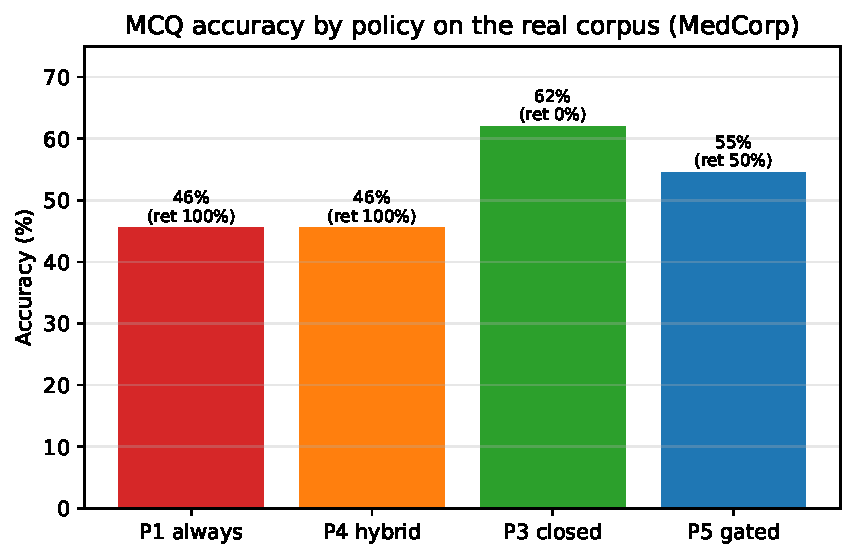
\includegraphics[width=0.75\linewidth]{results/figures/fig_medcorp_policies}
  \caption{MCQ accuracy by policy on the real corpus.}
  \label{fig:medcorp-policies}
\end{figure}
% WRITE: three claims, in this order:
%   (1) Selective beats always-retrieve: P5 \accPfiveMcq{} vs P1/P4 \accPoneMcq{},
%       at HALF the retrieval (\retPfiveMcq{}). State the cost halving as EXACT
%       (it is a count, not an estimate) and the accuracy gain as SUGGESTIVE
%       (\diffPfivePone{}pp, 95\% CI \diffPfivePoneCI{} — CROSSES ZERO).
%       This honesty is worth more than the claim would be.
%   (2) Closed-book P3 (\accPthreeMcq{}) still leads on MCQ.
%   (3) Open-ended INVERTS it: P5 (\f1PfiveOpen{}) > P3 (\f1PthreeOpen{}).
%       Retrieval helps exactly when the model does not already know — which is
%       precisely the condition the gate exists to detect. This MCQ-vs-open
%       split is itself a finding, not an inconsistency.
\todo{450 w — the three claims; cost-exact vs accuracy-suggestive framing.}

\section{Why Defaults Never Fired: Calibration Non-Transfer}
\label{sec:eval-calibration}
% BUDGET: 400 w
% SOURCE: week2 §prototype + week3 §calibration; fig_signals, fig_retrieval
\begin{figure}[t]
  \centering
  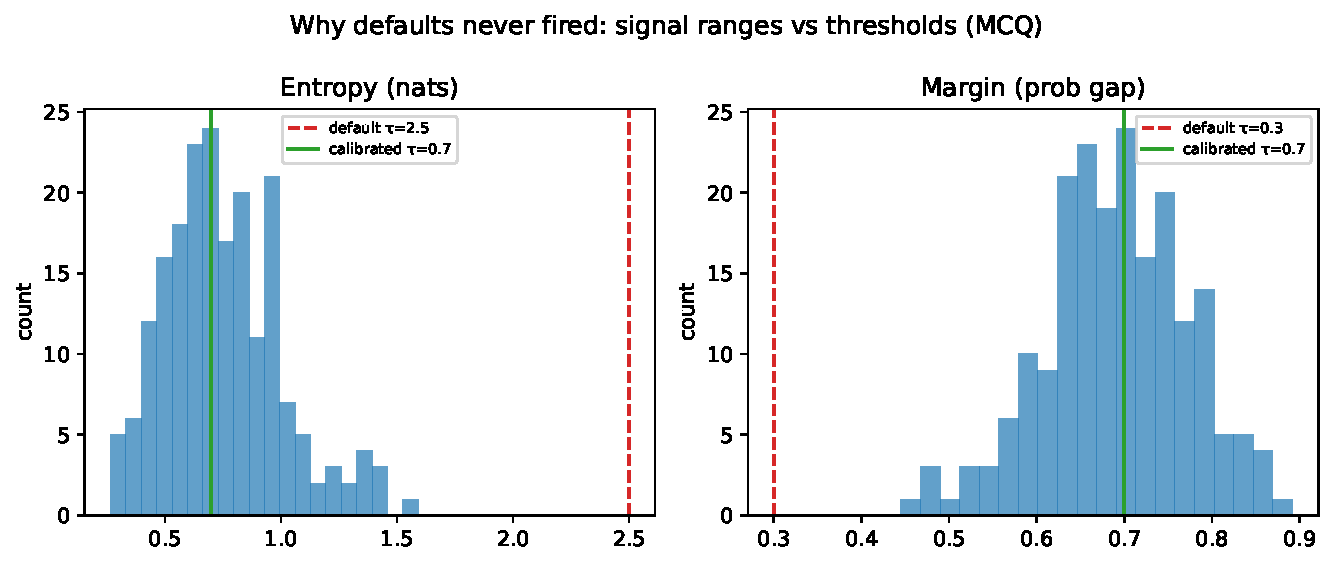
\includegraphics[width=\linewidth]{results/figures/fig_signals}
  \caption{Gate-signal distributions versus default and calibrated thresholds.}
  \label{fig:signals}
\end{figure}
% WRITE: at literature defaults (tau_H=2.5, tau_M=0.3) the gate retrieved on ZERO
% of 200 questions and P5 collapsed onto P3. Cause: on a 4-bit quantised 3B the
% draft distributions are sharply peaked — entropy never exceeds ~1.6 nats and
% margin never falls below ~0.45, so NEITHER threshold is physically reachable.
% Only the threshold-free probe ever voted retrieve (80/200), and one vote cannot
% carry a 2-of-3 majority. This is an EMPIRICAL FINDING, not a bug: thresholds
% calibrated on full-precision general-domain models do not transfer to a small
% quantised medical model. Recalibration is OFFLINE (replay the logged per-query
% signals at any threshold; seconds, not hours) => tau_H = tau_M = 0.70, giving
% \retPfiveMcq{} (MCQ) and \retPfiveOpen{} (open).
\todo{400 w — the zero-fire result and its cause; offline replay calibration.}

\section{The Corpus Was the Bottleneck}
\label{sec:eval-corpus}
% BUDGET: 300 w
\begin{figure}[t]
  \centering
  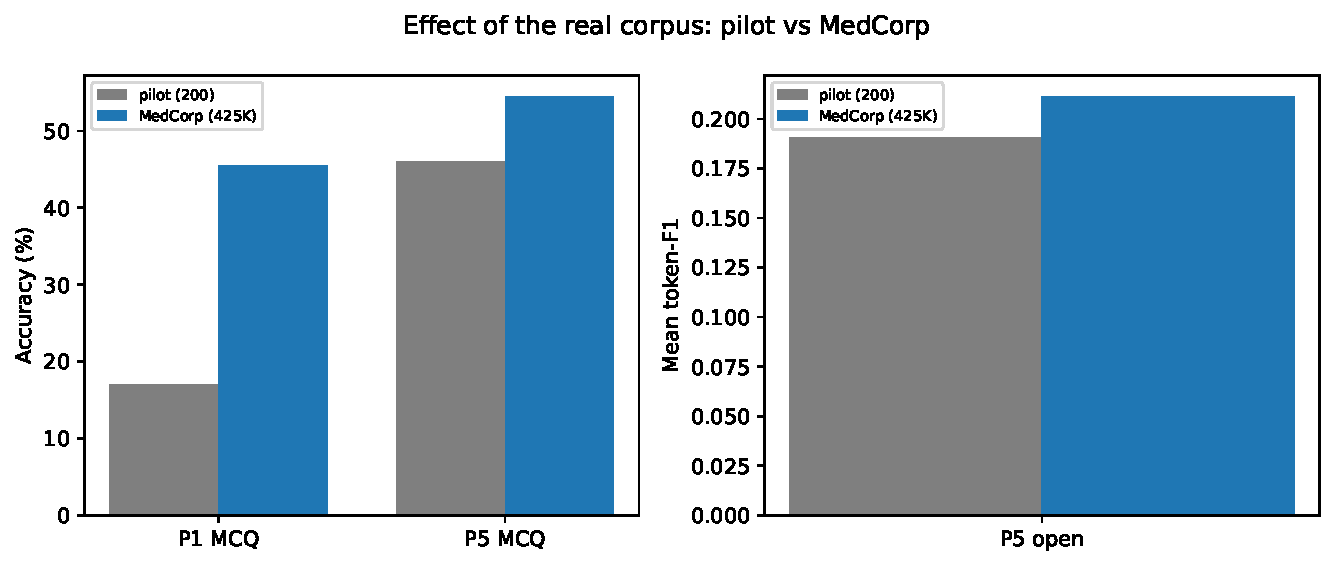
\includegraphics[width=\linewidth]{results/figures/fig_corpus_effect}
  \caption{Effect of replacing the 200-chunk pilot corpus with the 426K MedCorp corpus.}
  \label{fig:corpus-effect}
\end{figure}
% WRITE: on the pilot corpus P1 scored 17% and calibrated P5 DROPPED to 45.5% —
% i.e. once the gate started retrieving, it got worse. The lesson (state it as a
% general principle, it is your cleanest one): GATED RETRIEVAL INHERITS THE
% QUALITY OF THE CORPUS IT RETRIEVES FROM. The gate was functioning correctly;
% the corpus was empty of answers. Replacing it lifted P1 from 17% to
% \accPoneMcq{}, confirming the diagnosis retrospectively. Adaptive retrieval is
% only as safe as what it retrieves.
\todo{300 w — pilot collapse, the inheritance principle, the confirmation.}

\section{Retrieval as Distraction}
\label{sec:eval-distraction}
% BUDGET: 550 w  <-- **NEW. NOT IN ANY CURRENT CHAPTER. YOUR BEST MATERIAL.**
% SOURCE: p1_medcorp_mcq.jsonl + p3_mirage200.jsonl paired analysis;
%         p1_medcorp_mcq_chunks.jsonl + scripts/analyse_chunk_relevance.py
% WRITE, in this order — it is a whodunnit and the order matters:
%   (1) THE EFFECT. Paired P1-vs-P3 on identical questions: retrieval BREAKS 46
%       previously-correct answers and FIXES only 13. Net -33/200 (-16.5pp).
%       Harmful 3.5:1. This is why closed-book leads on MCQ — not model weakness.
%   (2) THE SYMPTOM. On those 46, P1's answers are ~15x LONGER than P3's
%       (274 vs 18 chars) and 26% are outright refusals ("the context does not
%       provide..."). The model stops answering and starts summarising.
%   (3) SUSPECT A — bad retrieval? Test it: measure gold-answer presence and
%       query-overlap in the retrieved chunks. Query-overlap is EQUAL across
%       groups (~0.14) => the retriever is NOT fetching off-topic junk.
%   (4) SUSPECT B — distraction? On broken questions the chunks are 2.4x LESS
%       ANSWER-BEARING (13% gold-in-chunk vs 31% on both-correct). So the model
%       receives text that is topically relevant but factually useless, cannot
%       distinguish "related" from "decisive", and ABANDONS a fact it already
%       knew.
%   (5) THE VERDICT — both, but not equally. Retrieval quality is a real ceiling
%       (headroom exists), but the FAILURE MODE is distraction. Worked example:
%       anatomy-020, gold "upper wall of right atrium"; the chunk correctly
%       discusses the SA node as pacemaker but never states its LOCATION; the
%       model writes a fluent, on-topic, wrong answer.
%   (6) THE PAYOFF, and lead the reader to it: if retrieval is poison on
%       questions the model already knows, then the value of a gate is not
%       efficiency — it is PROTECTION. Which sets up §5.6.
\todo{550 w — the distraction whodunnit. Include the anatomy-020 worked example.}

\section{The Protective Skip}
\label{sec:eval-protective}
% BUDGET: 300 w  <-- **NEW. THE SINGLE STRONGEST RESULT. NOT YET WRITTEN.**
% SOURCE: paired P5 gate decisions over the 46 "retrieval-poisoned" questions
% WRITE: take the 46 questions that retrieval breaks, and ask what P5's gate did.
%   - Where the gate SKIPPED retrieval: 19/19 correct = 100%.
%   - Where the gate RETRIEVED: 3/27 = 11%.
% The gate's skip decision is perfectly protective on exactly the subset where
% retrieval is harmful. This is the mechanistic justification for the whole
% method — and note carefully what it does NOT say: the gate is not identifying
% "easy" questions, it is identifying questions where the model's parametric
% answer is already right, which is a different and harder thing. Be careful not
% to overclaim from n=19; state it as a striking observation on a small subset,
% and put a CI on it.
\todo{300 w — 19/19 vs 3/27. State it plainly; caveat n=19; give a CI.}

\section{Gate Ablation: Does the Ensemble Earn Its Keep?}
\label{sec:eval-ablation}
% BUDGET: 400 w  <-- **NEW. Currently only in raw_logs/gate_variants_mcq.json.**
% WRITE: an examiner WILL ask "why three gates?". Answer it with data.
%   (a) SIGNAL CORRELATION: entropy and margin agree on 82% of decisions (both
%       are logit-derived — they are near-collinear). The probe agrees with
%       either only 55-58% => it measures something genuinely different.
%       Swing analysis: entropy decides 24% of ensemble outcomes, margin 26%,
%       probe 6%. The ensemble is not redundant.
%   (b) THE VARIANT SWEEP, replayed from logs (no new LLM calls):
%         majority_2of3 (shipped) : 54.5% acc, 49.5% retrieval
%         drop_margin             : 52.5% acc, 68.5% retrieval
%         probe_weighted          : 52.0% acc, 62.0% retrieval
%         probe_or_both_logit     : 52.0% acc, 62.0% retrieval
%   (c) THE HONEST BIT — MY HYPOTHESIS WAS REFUTED. The collinearity is real, so
%       I expected that up-weighting the probe (the independent signal) would
%       IMPROVE the ensemble. It does the opposite: every probe-boosting variant
%       retrieves MORE and scores WORSE. The probe OVER-triggers retrieval, and
%       the flat majority vote is PROTECTING the ensemble from it. This
%       corroborates §5.5 (retrieval-is-harmful) from a third, independent angle.
%   Report the refutation prominently. A stated hypothesis, tested and rejected,
%   with the reason understood, is worth more than a confirmed one.
% Determinism note: re-answering reproduced the logged answers exactly (3/3 at
% T=0), so the replay is faithful.
\todo{400 w — collinearity, the variant table, the refuted hypothesis.}

\section{Token-Level Entropy Attribution}
\label{sec:eval-attribution}
% BUDGET: 350 w  <-- figure EXISTS (fig_entropy_attribution), analysis does NOT.
\begin{figure}[t]
  \centering
  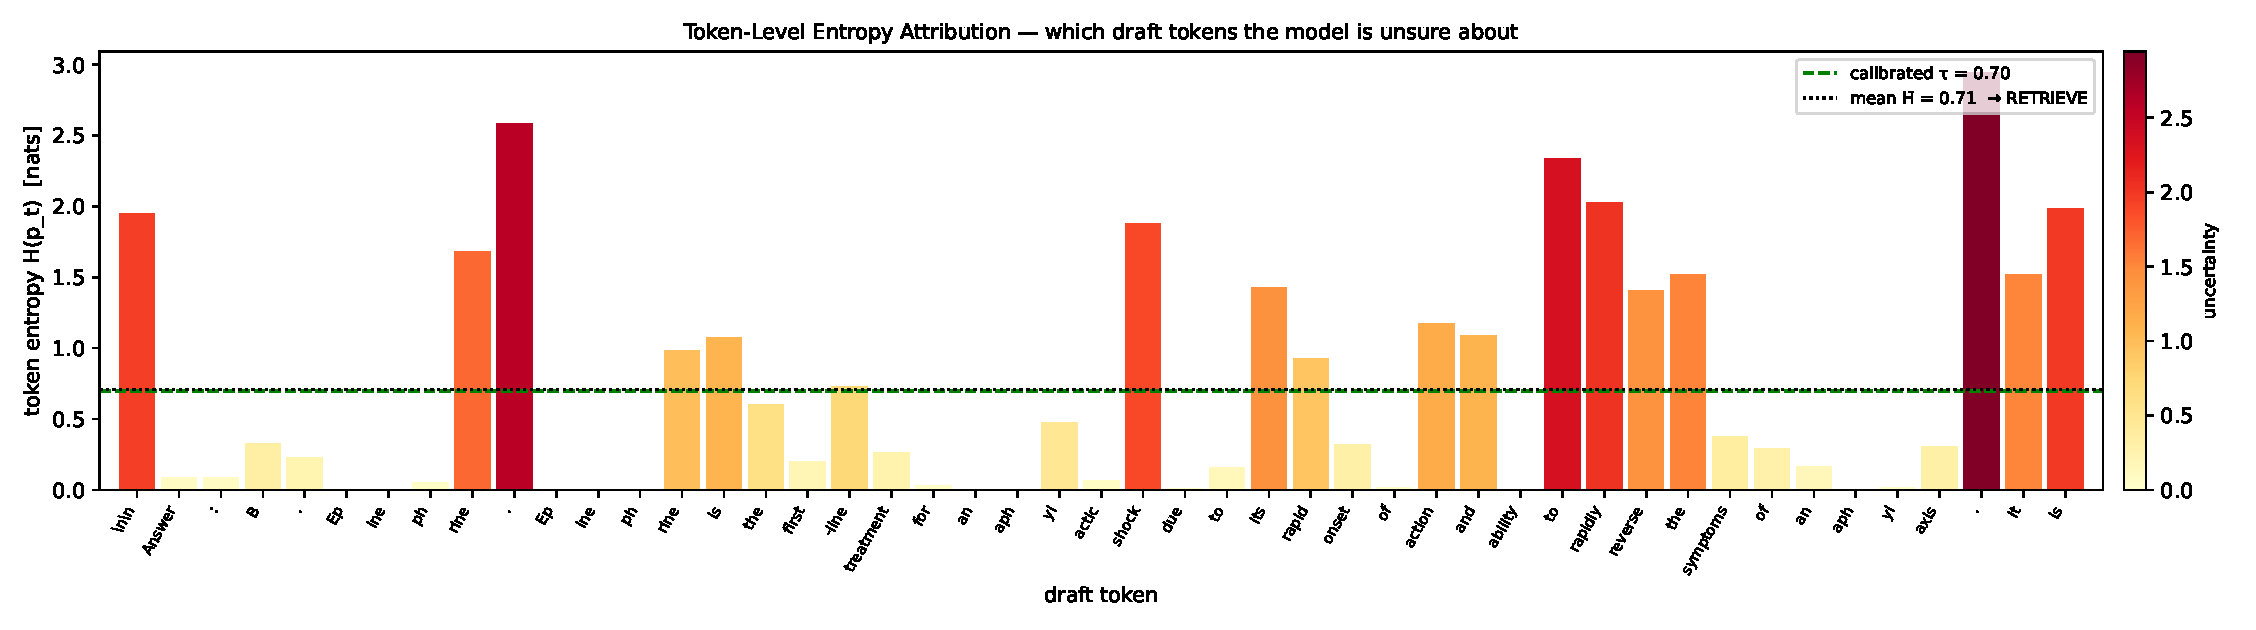
\includegraphics[width=\linewidth]{results/figures/fig_entropy_attribution}
  \caption{Per-token entropy across a drafted answer to a clinical question.}
  \label{fig:entropy-attribution}
\end{figure}
% WRITE: the gate logs the FULL per-token entropy array, so uncertainty can be
% localised to individual tokens rather than merely summarised. Worked example
% (anaphylaxis -> epinephrine): the mean H = 0.709 lands almost exactly on
% tau = 0.70, so the gate marginally RETRIEVES — a nice demonstration that it
% discriminates near the threshold. But the per-token view is the real result,
% and it is UNFLATTERING: the high-entropy tokens are FILLER and PHRASING
% ("\n\n", punctuation, "to", "is"), while the model is NEAR-CERTAIN on the
% clinically decisive tokens ("Ep/ine/ph/rine"). CONCLUSION, stated as a
% limitation of the METHOD and not hidden: raw token entropy largely measures
% PHRASING FREEDOM, not clinical-content uncertainty. This has a direct
% consequence — a content-aware variant (entropy restricted to content tokens,
% or attention-weighted) is the obvious next design, and it is future work.
% This is your most distinctive asset. Do not bury it, and do not spin it.
\todo{350 w — attribution; report the unflattering filler-token finding honestly.}

\section{Risk Stratification and the Safety Envelope}
\label{sec:eval-envelope}
% BUDGET: 450 w
% SOURCE: results/tables/tab_risk.tex (\input); fig_safety_envelope
% AUTO-GENERATED by scripts/generate_tables.py -- DO NOT EDIT.
% Regenerate with: python scripts/generate_tables.py
% Every number is computed from results/raw_logs/ via evaluation.loading.
% git b3a9d01 | 2026-07-13 13:27
\begin{table}[t]
  \centering
  \begin{tabular}{lccc}
    \toprule
    & \multicolumn{3}{c}{Accuracy \% [95\% Wilson CI]} \\
    \cmidrule(lr){2-4}
    Policy & Low ($n=28$) & Medium ($n=166$) & High ($n=6$) \\
    \midrule
    P1 always-retrieve & 28.6\% [15, 47] & 47.6\% [40, 55] & 66.7\% [30, 90] \\
    P4 hybrid & 28.6\% [15, 47] & 47.6\% [40, 55] & 66.7\% [30, 90] \\
    P3 closed-book$^\dagger$ & 64.3\% [46, 79] & 60.8\% [53, 68] & 83.3\% [44, 97] \\
    P5 gated (calib.) & 50.0\% [33, 67] & 55.4\% [48, 63] & 50.0\% [19, 81] \\
    \bottomrule
  \end{tabular}
  \caption{Multiple-choice accuracy by clinical risk level, with 95\% Wilson score
  intervals. The high-risk stratum contains only $n=6$ questions, giving intervals
  roughly $\pm$30 percentage points wide: \emph{no comparison between policies at high
  risk is statistically meaningful in this evaluation}. The medium stratum
  ($n=166$) is where the headline comparison actually rests, and even there the
  intervals overlap.}
  \label{tab:risk}
\end{table}

\begin{figure}[t]
  \centering
  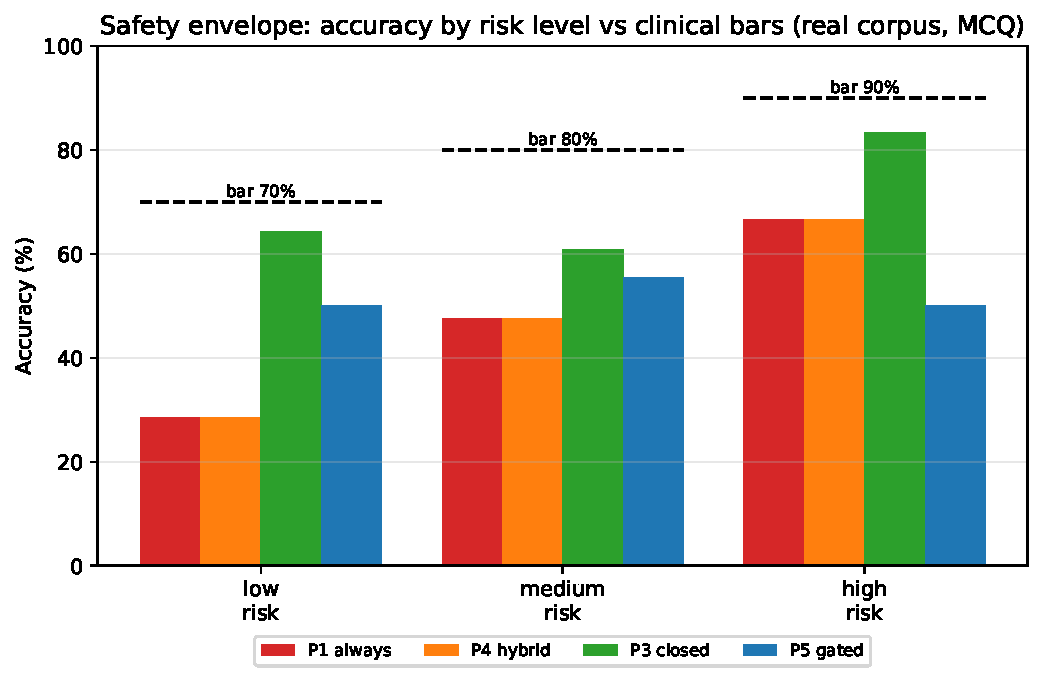
\includegraphics[width=\linewidth]{results/figures/fig_safety_envelope}
  \caption{Safety envelope: policy accuracy by clinical risk level against the
           stipulated clinical bars. No cell clears its bar.}
  \label{fig:safety-envelope}
\end{figure}
% WRITE, and DO NOT APOLOGISE:
%   - The envelope is EMPTY: no policy clears even the \barLow{} low-risk bar.
%     The best result on the benchmark, closed-book P3 at \accPthreeMcq{}, is
%     \gapToLowBar{}pp short.
%   - Reframe this as the CONTRIBUTION, not the shortfall: this quantifies the
%     DISTANCE between a state-of-practice offline small-model medical RAG system
%     and clinical acceptability. That number is genuinely useful and nobody else
%     has published it for this configuration. A dissertation that says "we are
%     8 points short and here is exactly why" is stronger than one that claims
%     clinical readiness it cannot support.
%   - It is now a MODEL-CAPABILITY ceiling, not a corpus one: retrieval has been
%     shown to work and the corpus demonstrably contains the answers.
%   - STATISTICAL HONESTY: the high-risk stratum has n=6 => 95% Wilson CIs of
%     roughly +/-30pp. NO comparison between policies at high risk is meaningful.
%     Say this in bold. The headline comparison actually rests on the medium
%     stratum (n=166), and even there the intervals overlap.
\todo{450 w — empty envelope as a quantified distance; hard caveat on n=6.}

\section{Cost, Latency and the Trade-off Frontier}
\label{sec:eval-cost}
% BUDGET: 300 w
\begin{figure}[t]
  \centering
  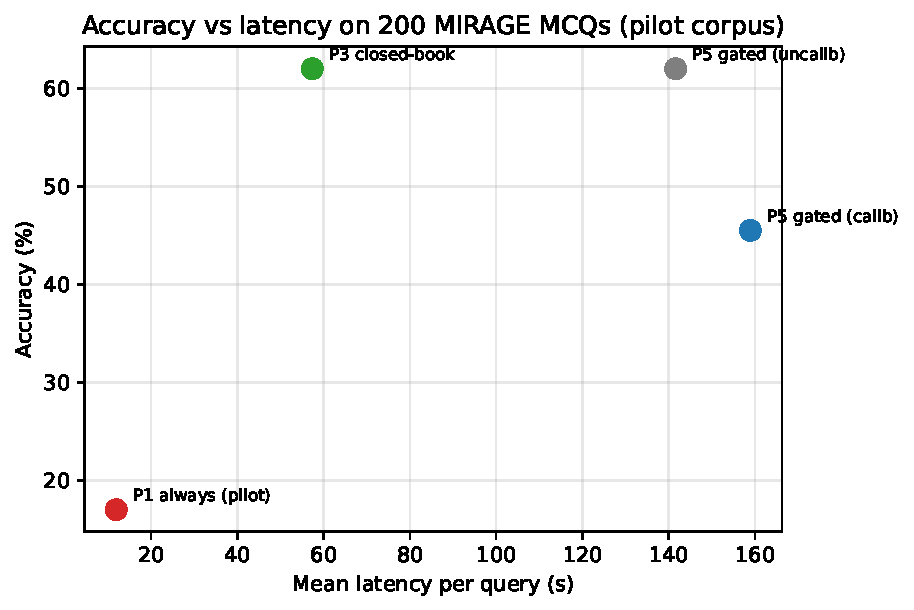
\includegraphics[width=0.8\linewidth]{results/figures/fig_pareto}
  \caption{Accuracy versus mean latency per query.}
  \label{fig:pareto}
\end{figure}
% WRITE: the uncomfortable engineering truth, stated plainly: P5's latency
% (\latPfiveMcq{}) EXCEEDS P1's (\latPoneMcq{}) because the ensemble issues three
% extra drafts (entropy/margin draft + two probe drafts) BEFORE the answer. So
% the gate as implemented saves RETRIEVAL calls (halved — exact) but does NOT
% save wall-clock time on CPU. Do not hide this behind the retrieval-rate number.
% Then the constructive response, which is real: the probe's two drafts dominate,
% and the entropy and margin signals come from the SAME draft — so merging the
% draft calls (5 LLM calls -> 4) and a probe-free logit-only configuration are
% the obvious optimisations, quantified in Future Work. The cost story today is
% "fewer retrievals, more generation"; whether that is a win depends on whether
% retrieval or generation dominates the deployment — on a large corpus over slow
% storage, it is retrieval; on this laptop, it is generation. Say exactly that.
\todo{300 w — admit P5 is SLOWER in wall-clock; explain when the trade is worth it.}

% =====================================================================
\chapter{Discussion}
\label{ch:discussion}
% CHAPTER BUDGET: 1,500 words
% =====================================================================

\section{What the Findings Mean Together}
\label{sec:disc-synthesis}
% BUDGET: 450 w
% WRITE: assemble the chain into ONE argument, do not just re-list the results:
%   Retrieval is not a free safety net. On questions the model already answers
%   correctly, injecting topically-relevant-but-not-decisive context makes it
%   WORSE (3.5:1 harmful). Therefore the value of a retrieval gate is not
%   primarily efficiency — the framing the adaptive-RAG literature has mostly
%   adopted — but PROTECTION. The 19/19 protective-skip result is the sharpest
%   evidence for this reframing. It also explains, without special pleading, why
%   closed-book wins on MCQ and loses on open-ended: the gate's real job is to
%   detect the boundary of parametric knowledge, and MCQ sits inside it while
%   PubMedQA sits outside it.
\todo{450 w — the synthesis: gating is PROTECTION, not just efficiency.}

\section{Limitations and Threats to Validity}
\label{sec:disc-limitations}
% BUDGET: 600 w — BE COMPREHENSIVE. Naming your own weaknesses first is what
% separates a Distinction from a Merit. Cover ALL of these:
%   - STATISTICAL POWER: n=200, single seed. Headline gap +\diffPfivePone{}pp has
%     95% CI \diffPfivePoneCI{} — crosses zero. High-risk stratum n=6 (+/-30pp).
%     Say plainly: this study is not powered to establish the accuracy claim; the
%     retrieval-cost claim is a count and is exact.
%   - SINGLE MODEL: everything rests on one quantised Llama-3.2-3B.
%     "Calibration does not transfer" and "selective beats always" are
%     single-model observations until replicated. (State whether the Qwen run
%     happened; if it did, this limitation shrinks — update accordingly.)
%   - HARDWARE TIERS NOT PHYSICALLY TESTED. The tier-degradation MECHANISM is
%     implemented and unit-tested, but only the medium tier was actually run.
%     Do not imply three devices were benchmarked. (The original project plan
%     promised this; the honest thing is to say what was and was not delivered.)
%   - BENCHMARK NARROWNESS: MCQ = MIRAGE/MMLU only; open-ended = PubMedQA only.
%     MIRAGE is entirely multiple-choice. The intended RAGCare-QA path was dead.
%   - METRIC LIMITS: token-F1 on paragraph answers is harsh in absolute terms
%     (0.19-0.22) — report RELATIVE differences only. Energy is a codecarbon
%     SOFTWARE ESTIMATE, not a hardware RAPL measurement.
%   - RISK TAGGER: rule-based keyword heuristic. Auditable by design (a learned
%     classifier would obscure the basis of a safety-relevant label and there is
%     no training data for it), but it has recall gaps on implicitly high-risk
%     questions. That gap is partly WHY the high-risk stratum is only n=6.
%   - SAFETY BARS ARE STIPULATED (70/80/90), not derived from clinical practice.
\todo{600 w — the full threat list. Do not soften any of it.}

\section{Implications for Offline Clinical Deployment}
\label{sec:disc-deployment}
% BUDGET: 450 w
% WRITE: what a practitioner should actually take away.
%   - At the 3B scale, DO NOT deploy for clinical decision support. The safety
%     envelope is empty; the honest output of this work is a distance, not a
%     product. State this bluntly — it is the responsible finding.
%   - Where the method IS useful today: cost-and-safety-aware ROUTING in
%     offline/on-prem settings (data-sovereignty constraints, low connectivity,
%     edge devices), where retrieval is expensive and a model that "knows it
%     knows" can be trusted to skip it.
%   - Interpretability as the deployable asset: the per-token attribution
%     surfaces WHERE the model was uncertain — trust and auditability matter more
%     in regulated healthcare than a small accuracy delta. (Note the honest
%     caveat from §5.8: current entropy attribution highlights phrasing, not
%     content — so this is a promising DIRECTION, not a finished feature.)
\todo{450 w — do not deploy at 3B; where routing + attribution are genuinely useful.}

% =====================================================================
\chapter{Legal, Social and Ethical Considerations}
\label{ch:lsep}
% CHAPTER BUDGET: 1,200 words
% Required by the KCL rubric (10%). This is the cheapest 10% in the marking
% scheme and a medical-AI project makes it easy. Do not phone it in, and do not
% write generic AI-ethics filler — tie EVERY point to a specific design decision
% you actually made.
% =====================================================================

\section{Patient Safety and Clinical Liability}
\label{sec:lsep-safety}
% BUDGET: 400 w
% WRITE: the asymmetry of harm (an unnecessary retrieval costs seconds; a
% confidently wrong drug-interaction answer costs a patient) is not a rhetorical
% flourish — it is ENCODED IN THE DESIGN: the ensemble is deliberately biased
% toward retrieving when signals disagree. Then the hard part: an empty safety
% envelope means this system MUST NOT be used for clinical decision support, and
% the dissertation says so. Discuss liability (who is responsible for a wrong
% answer — the model, the deployer, the clinician?), automation bias (a fluent,
% confidently-worded wrong answer is MORE dangerous than an obviously uncertain
% one — and §5.5 showed retrieval makes answers longer and more fluent while
% making them WRONG), and the regulatory posture (UK MHRA / EU AI Act treat
% clinical decision support as high-risk; this is a benchmark, not a device).
\todo{400 w — harm asymmetry as a DESIGN decision; liability; automation bias.}

\section{Privacy, Data Governance and Sovereignty}
\label{sec:lsep-privacy}
% BUDGET: 350 w
% WRITE: the offline, CPU-only architecture is a PRIVACY ARCHITECTURE, not just a
% cost one — no query, no patient context, and no retrieved passage ever leaves
% the device, which is what makes the system viable where GDPR/NHS data-governance
% rules forbid sending clinical text to a third-party API. Contrast explicitly
% with cloud RAG. Then the honest limits: the corpus itself (PubMed, textbooks)
% is public, so this project handled NO patient data; the PhysioNet-credentialed
% EHR datasets in the original plan were NOT used. Say so — claiming privacy
% engineering you did not have to do would be dishonest.
\todo{350 w — offline as privacy architecture; concede no patient data was handled.}

\section{Bias, Equity and Access}
\label{sec:lsep-bias}
% BUDGET: 250 w
% WRITE: the corpus is Western textbook + PubMed — its epidemiological and
% demographic assumptions are baked into every retrieved passage, and a gate that
% skips retrieval inherits the MODEL's biases instead. Neither path is neutral.
% Then the equity argument that actually motivates the whole project: an offline
% CPU-only system is precisely the one that can run where GPUs, budgets and
% connectivity do not exist (LMIC clinics, rural practice) — but see §7.1, at 3B
% it is not yet safe to do so, and shipping an unsafe system to under-resourced
% settings would be worse than shipping nothing.
\todo{250 w — corpus bias vs parametric bias; the access argument and its danger.}

\section{Environmental Cost}
\label{sec:lsep-energy}
% BUDGET: 200 w
% WRITE: per-query energy (codecarbon estimate — say it is an estimate). The
% honest accounting: the gate HALVES retrieval calls but ADDS draft generations,
% so on this hardware it is not currently an energy win (cf. §5.10). The energy
% case for gating is real but conditional — it depends on retrieval dominating
% the cost profile, which it does on large corpora over slow storage and does not
% on this laptop. Do not claim a green win you did not measure.
\todo{200 w — energy honestly; do not claim an unearned green win.}

% =====================================================================
\chapter{Conclusion and Future Work}
\label{ch:conclusion}
% CHAPTER BUDGET: 900 words
% =====================================================================

\section{Summary of Contributions}
\label{sec:conc-summary}
% BUDGET: 400 w
% WRITE: restate C1-C6 from §1.4, now with the numbers attached and each one
% earned by a specific chapter. Keep the claims exactly as strong as the evidence
% supports — cost halving EXACT, accuracy gain SUGGESTIVE, envelope EMPTY.
% One line that should appear somewhere: the most useful result in this thesis is
% a negative one — retrieval, the field's default remedy for hallucination, made
% this model WORSE on 46 of 200 questions, and the gate's value is that it knows
% when not to use it.
\todo{400 w — contributions with numbers; keep every claim exactly as strong as its evidence.}

\section{Future Work}
\label{sec:conc-future}
% BUDGET: 500 w — order by RATIO OF VALUE TO EFFORT, and be specific enough that
% someone could actually pick each one up:
%   1. SCALING STUDY (prereqs already built: chat-format abstraction verified
%      byte-identical, Qwen 7B/14B configs, smoke test, Colab notebook). Does
%      "selective beats always" and "calibration non-transfer" survive a larger
%      model? Highest-value, lowest-risk.
%   2. CONTENT-AWARE ENTROPY. §5.8 showed raw token entropy fires on PHRASING,
%      not clinical content. Restrict entropy to content tokens, or weight by
%      attention to the question's clinical terms. This directly attacks the
%      method's biggest measured weakness.
%   3. RETRIEVAL-AWARE GATING. §5.5 showed the failure is topically-relevant,
%      non-answer-bearing chunks. A post-retrieval gate ("having seen the chunks,
%      are they DECISIVE?") could reject a retrieval after the fact — the current
%      gate must commit before it sees anything.
%   4. COST OPTIMISATION. Merge the entropy/margin draft (5 LLM calls -> 4);
%      evaluate a probe-free logit-only configuration. §5.10 shows the ensemble's
%      latency, not its retrieval rate, is the binding cost.
%   5. POWER. n=200 is not enough. The full 7,663-question MIRAGE benchmark, and
%      a purposely balanced high-risk stratum (the current n=6 is the single
%      weakest point in the safety analysis).
%   6. DEPLOYMENT: human-in-the-loop UI surfacing the gate decision and the
%      per-token uncertainty; physical benchmarking on real 4GB/16GB devices.
\todo{500 w — six directions, ordered by value-to-effort, each specific enough to act on.}

% =====================================================================
\bibliographystyle{plainnat}
\bibliography{references}
% !! references.bib is currently an 8-entry STUB with [TODO verify] fields.
% Needed (~15-20): Lewis RAG; Asai Self-RAG (ICLR'24); Jeong Adaptive-RAG
% (NAACL'24); SmartRAG (ICLR'25); TARG (verify arXiv id); Mallen (ACL'23);
% Xiong MIRAGE/MedRAG (ACL Findings'24); Singhal Med-PaLM (Nature'23);
% Jin PubMedQA; Kadavath (2022); Wang self-consistency (2023); Guo ECE (ICML'17);
% Gao ALCE (EMNLP'23); Robertson & Zaragoza BM25; Reimers sentence-transformers;
% Johnson FAISS; Strubell (ACL'19); Wilkins (HotCarbon'24); llama.cpp; Llama-3.

\appendix
\chapter{Reproducibility Artefacts}
% NOT counted in the 15,000 words. Include:
%   - exact run commands per experiment + the config file used
%   - JSONL RunRecord schema (one annotated example record)
%   - the generated numbers.tex, showing every reported figure and its source log
%   - test inventory (180+) and how to run the suite without the model
%   - corpus build parameters (sources, 425,847 chunks, index sizes)
\todo{Appendix — run commands, JSONL schema, numbers.tex, test inventory, corpus params.}

\end{document}

% =====================================================================
%  WORD BUDGET
% ---------------------------------------------------------------------
%   Abstract                              250
%   1 Introduction                      1,500
%   2 Background & Related Work         2,500
%   3 Methodology & Design              2,500
%   4 Implementation                    2,000
%   5 Evaluation & Results              3,000   <-- write this FIRST
%   6 Discussion                        1,500
%   7 Legal, Social & Ethical           1,200
%   8 Conclusion & Future Work            900
%                                      -------
%                                      15,350   (~15,000 target)
%
%  Existing drafts ~6,000 real words (week1-4) map onto Ch3/Ch4/Ch5.
%  New writing needed: ~9,000 words (Ch1, Ch2, Ch6, Ch7, Ch8 + the five
%  unwritten Ch5 analyses, which are the highest-value words in the thesis).
%
%  RE-THREADING NOTE: week1-4 are chronological SPRINT LOGS ("Week 2 delivered
%  X but left three gaps..."). A thesis chapter is organised by CONCEPT, not by
%  time. When migrating, keep the reasoning and the equations; delete every
%  "this sprint", "Week N", "the prototype". Change the tense, not the argument.
% =====================================================================
